\chapter{Sense Amplifier analyse}
\label{sensamp}
Een sense amplifier versterkt kleine signaalverschillen tot rail-tot-rail signalen. Aangezien de uitgangsignalen hiervan ook de uitgelezen bits zijn van het geheugen, is het bovenal belangrijk dat dit op een correcte manier gebeurt, ondanks variabiliteit.
In dit hoofdstuk wordt de sense amplifier dus ook wat dieper onderzocht. Uiteindelijk wordt een SA ontwerpen die functioneert op een robuuste manier en die ook voldoende snel en laagenergetisch is.

\section{Types SA}
Er bestaan heel wat verschillende soorten sense amplifiers, traditioneel kunnen die op twee verschillende manieren geclassificeerd worden. Enerzijds kan men onderscheid maken tussen differentiële en niet-differentiële SA. Anderzijds maakt men onderscheid tussen voltage SA en current SA. Een voorbeeld van een niet-differentiële SA is een inverter. De drempelspanning waarbij de inverter schakelt wordt bepaald door de groottes van de transistoren. Deze architectuur is echter bijzonder susceptibel aan globale variabelen zoals temperatuur en voedingsspanning. Een dergelijk probleem kan opgelost worden door een referentiesignaal dat gelijke variaties ervaart door deze globale schommelingen als het datasignaal. Voor een dergelijke architectuur zijn uiteraard differentiële SA nodig. Current en voltage SA verschillen in ingangsimpedantie: bij een hoge ingangsimpedantie spreekt men van voltage-sensing, bij een lage impedantie spreekt men van current-sensing. Voorbeelden van voltage- en current-mode sense amplifiers zijn geïllustreerd in figuren \ref{fig:voltagemodesa} en \ref{fig:currentmodesa}. Voor de architectuur van dit werk waarbij de data- en referentiesignalen opgewekt worden door een spanningsdeling met eigen gekozen lastimpedantie, is een SA nodig met een grote ingangsimpedantie.

\begin{figure}
  \centering
  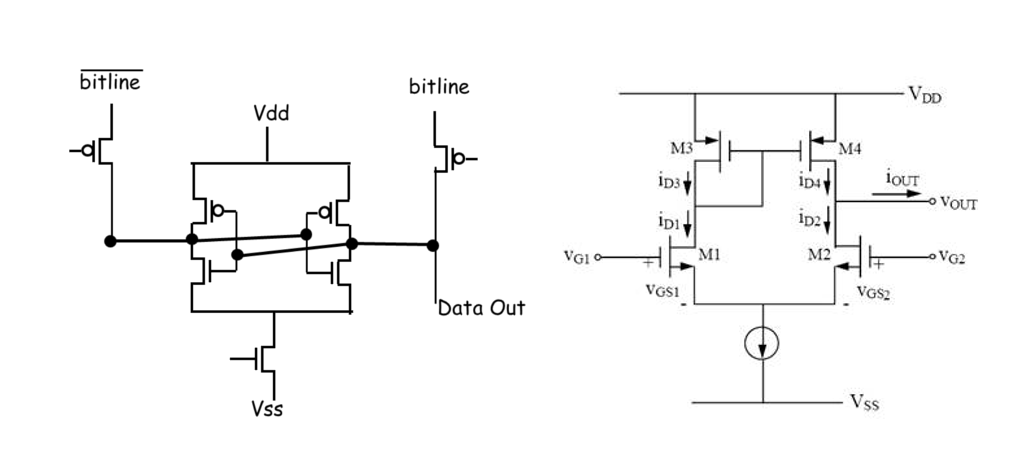
\includegraphics[width=\textwidth]{../fig/hfdstk-sensamp-voltagemode.png}
  \caption[Voltage mode sense amplifiers]{Voltage mode sense amplifiers}
  \label{fig:voltagemodesa}
\end{figure}
\begin{figure}
  \centering
  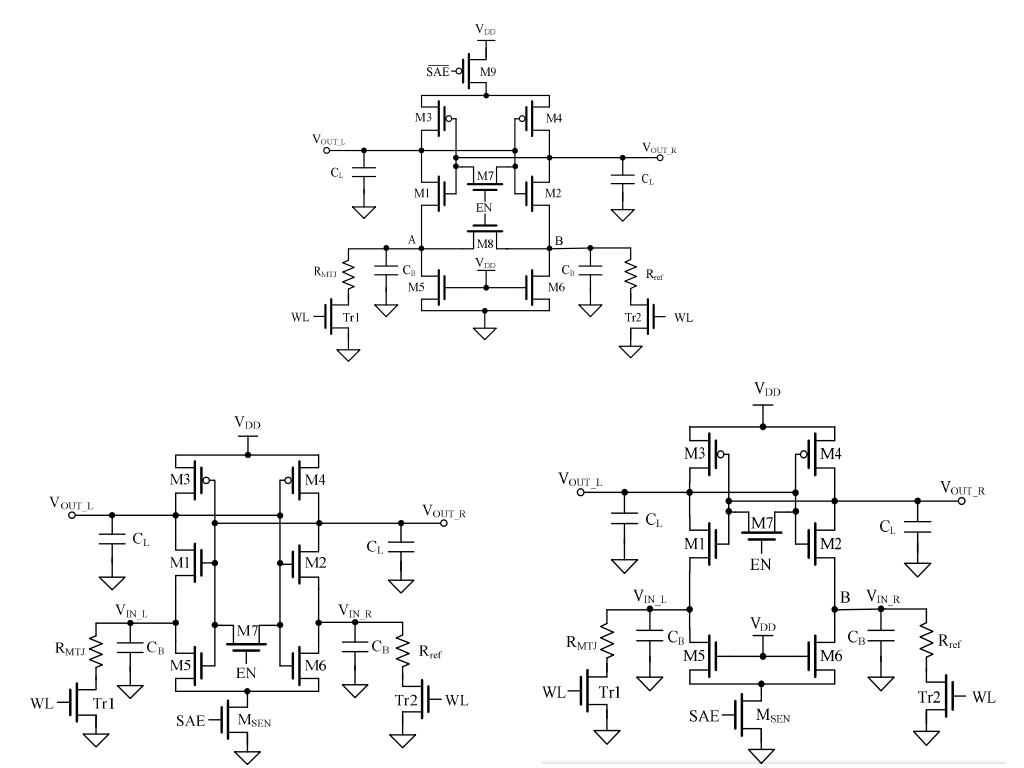
\includegraphics[width=\textwidth]{../fig/hfdstk-sensamp-currentmode.png}
  \caption[Current mode sense amplifiers]{Current mode sense amplifiers, reproduced from\cite{5548588}}
  \label{fig:currentmodesa}
\end{figure}

\begin{figure}
  \centering
  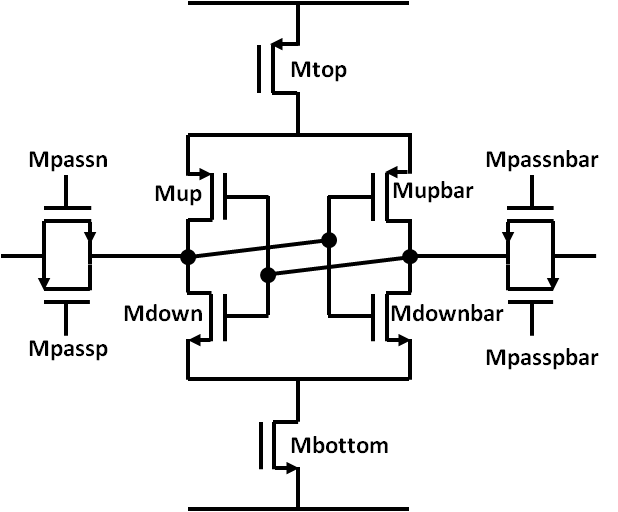
\includegraphics[scale=0.4]{../fig/hfdstk-sensamp-ourSA.png}
  \caption[De drain-input latch-type SA]{De drain-input latch-type SA}
  \label{fig:ourSA}
\end{figure}

Omwille van eenvoudigheid en goede performantie\cite{Cos09} wordt er in wat volgt voortgewerkt met de SA van figuur \ref{fig:ourSA}.


\section{Offsetspanning}
Een ideale sense amplifier zal voor elke twee ingangssignalen correct versterken, tenzij de signalen dezelfde zijn, waarna de SA in een metastabiele toestand belandt. In de praktijk is er echter wegens variabiliteit een limiet voor het ingangsspanningsverschil waarbij er correct versterkt wordt. Deze limiet heet de offsetspanning en wordt geïllustreerd in figuur \ref{fig:offset}. De offsetspanning van een SA is in de ontwerpfase een stochastische variabele met gemiddelde 0V, pas nadat een chip gefabriceerd is ligt de offsetspanning definitief vast [al kan het zijn dat deze met de tijd nog verandert].
Er zijn 2 manieren waarop men de offsetspanning van een systeem kan aanpakken: ofwel ontwerp je het systeem zodanig dat het verschil van de ingangssignalen van de SA groot genoeg is zodat ze [in 99,9\% van de gevallen] niet groter is dan de offsetspanning, ofwel bouw je een mechanisme in waarbij je na fabricatie de offsetspanning meet en vervolgens compenseert. In dit werk is gekozen voor het eerste.
Hiervoor is het wel belangrijk te onderzoeken wat de verdeling is van de offsetspanning, dit wordt gedaan in de volgende sectie.

\begin{figure}
  \centering
  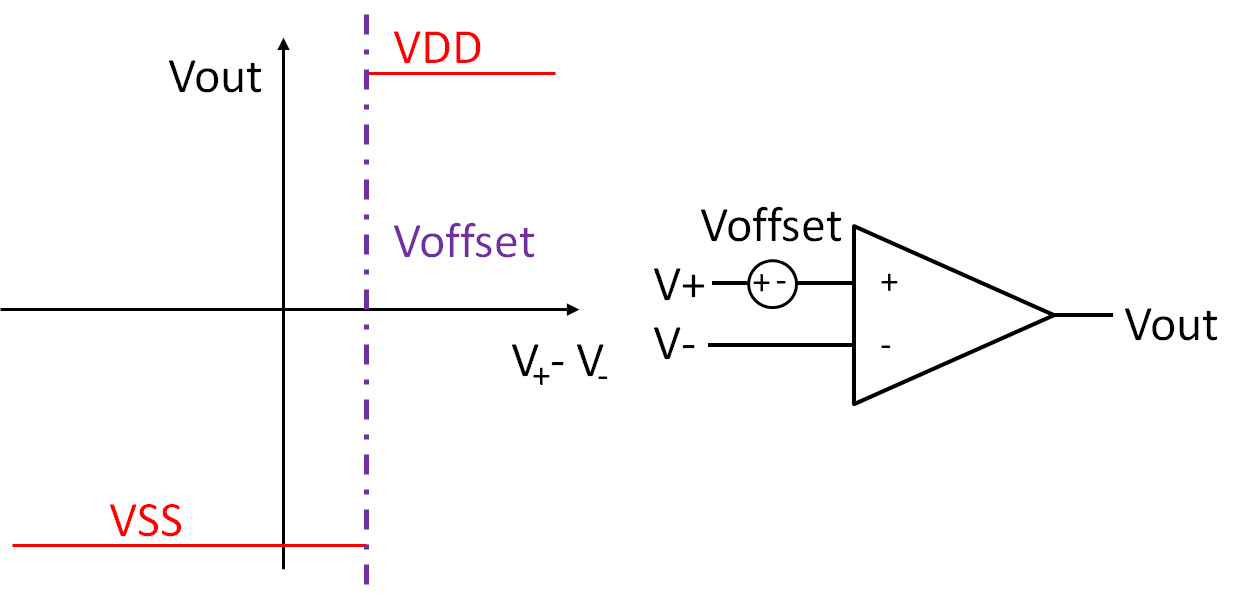
\includegraphics[scale=0.4]{../fig/hfdstk-sensamp-offset.png}
  \caption[SA offsetspanning]{Illustratie van offsetspanning}
  \label{fig:offset}
\end{figure}

\section{Sensitiviteitsanalyse}
De SA wordt gerealiseerd als een circuit met transistors. Elke transistor heeft 2 stochastische parameters met een normale verdeling, nl. $\Delta V\textsubscript{t}$ en $\Delta \beta$. De spreiding van deze verdelingen is gekend: $\sigma_{\Delta V_{t}} = \frac{A\textsubscript{V\textsubscript{t}}}{\sqrt{W L}}$ en $\sigma_\frac{{\Delta \beta}}{\beta} = \frac{A_{\beta}}{\sqrt{W L}}$. Met een sensitiveitsanalyse kan men uit deze standaardafwijkingen de standaardafwijking van de offsetspanning $\sigma_{V_{offset}}$ berekenen. Hierbij wordt verondersteld dat de stochastische variabele $V_{offset}$ een lineaire combinatie is van de normaal verdeelde afwijkingen $(\Delta V_{t})_{i}$ en $(\frac{\Delta_{\beta}}{\beta})_{i}$: $V_{offset}=\sum\limits_{i=1}^{N} a_{i} (\Delta V_{t})_{i} + b_{i} (\frac{\Delta_{\beta}}{\beta})_{i}$.
$a_{i}$ en $b_{i}$ zijn de gevoeligheden van de offset naar de variatieparameters: $a_{i}=\frac{\partial V_{offset}}{\partial (\Delta V_{t})_{i}}$ en $b_{i}=\frac{\partial V_{offset}}{\partial (\frac{\Delta_{\beta}}{\beta})_{i}}$.
Voor een dergelijke variabele geldt dan: $\sigma_{V_{offset}}=\sqrt{\sum\limits_{i=1}^{N} a_{i}^{2} (\sigma_{\Delta V_{t}})_{i}^{2} + b_{i}^{2} (\sigma_{\frac{\Delta_{\beta}}{\beta}})_{i}^{2}}$.

Er moet wel geverifieerd worden of de stelling dat er een lineaire afhankelijkheid is tussen $V_{offset}$ en de variatieparameters gegrond is.
Dit kan gedaan worden aan de hand van een analyse waarbij elke variatieparameter afzonderlijk gesweept wordt, een noodzakelijke maar niet voloende vereiste.

\subsection{Sensitiviteitsanalyse op een minimale SA}
In figuur \ref{fig:min-sensanalysis} wordt het resultaat getoond voor een dergelijke analyse bij een SA met minimale afmetingen, merk op dat de richtingscoëfficient van deze curves gelijk is aan $a_{i} (\Delta V_{t})_{i}$ en $b_{i} (\frac{\Delta_{\beta}}{\beta})_{i}$.  In tabel \ref{tab:min-sensanalysis} worden de resultaten en de resulterende standaardvariatie van de SA getoond.
Er moet opgemerkt worden dat er bij deze simulatie slechts gesweept werd voor de variatieparameters van -4$\sigma$ tot 4 $\sigma$. Dit is om de reden dat voor de minimale transistoren de standaardvariatie het grootst is. In de Spectre-simulaties zouden transistoren voor te grote negatieve $\beta$-mismatch stroom leveren in de omgekeerde richting. Deze situatie zal fysisch nooit optreden.

\begin{figure}[!ht]
\centering
\subfloat[Vt-mismatch]{ 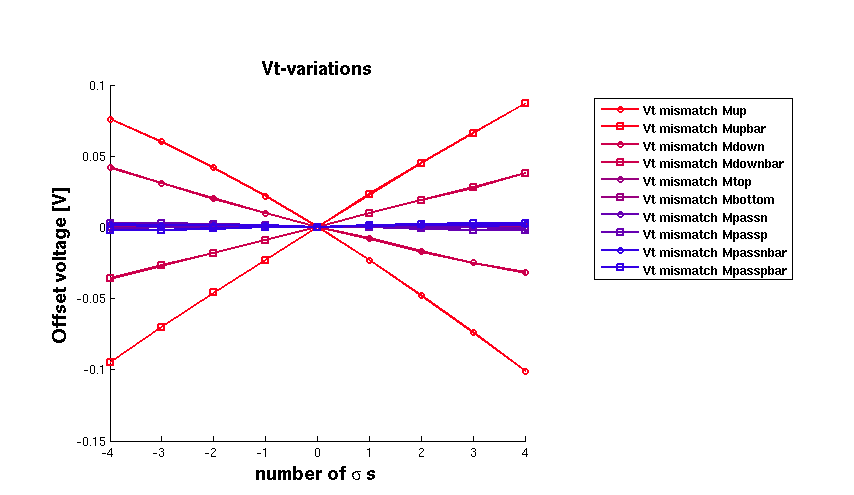
\includegraphics[width=0.9\textwidth] {../fig/hfdstk-sensamp-vt-sensitivity.png}} \\
\subfloat[$\beta$-mismatch]{ 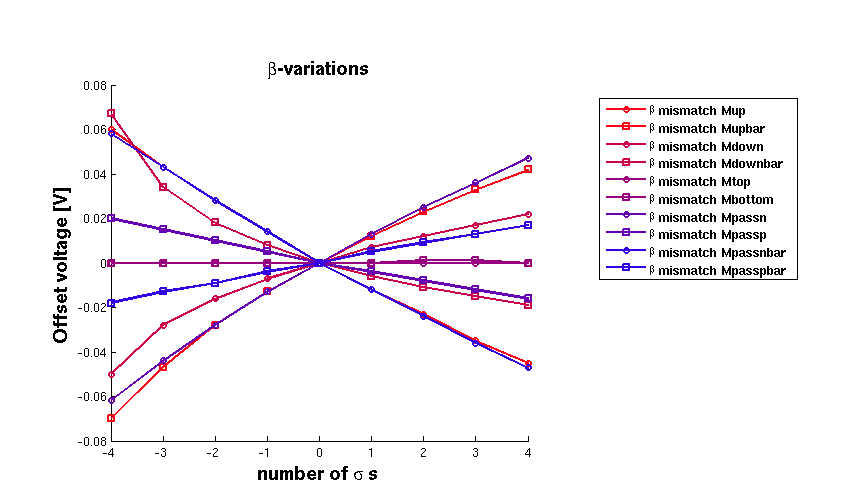
\includegraphics[width=0.9\textwidth] {../fig/hfdstk-sensamp-b-sensitivity.png}}

\caption[Sensitiviteitsresultaten: offsetspanning i.f.v. mismatchvariabelen]{Sensitiviteitsresultaten: offsetspanning i.f.v. mismatchvariabelen}
\label{fig:min-sensanalysis}
\end{figure}


\begin{table}
\begin{tabular}{cccccc}
\hline 
Transistor & Parameter & Richtingscoëfficiënt [$\frac{mV}{\sigma}$] & W [nm] & L [nm] & $\sigma$ \\ 
\hline 
Mupbar & Vt & 22.7 & 100 & 45 & 37.3mV \\ 
Mup & Vt & -22.3 & 100 & 45 & 37.3mV \\ 
Mupbar & $\beta$ & 13.6 & 100 & 45 & 17.9\% \\ 
Mpassn & $\beta$ & 13.5 & 100 & 45 & 29.8\% \\ 
Mpassbarn & $\beta$ & -13.1 & 100 & 45 & 29.8\% \\ 
Mup & $\beta$ & -13.0 & 100 & 45 & 17.9\% \\ 
Mdownbar & $\beta$ & -9.4 & 100 & 45 & 29.8\% \\ 
Mdown & Vt & -9.3 & 100 & 45 & 42.0mV \\ 
Mdownbar & Vt & 9.2 & 100 & 45 & 42.0mV \\ 
Mdown & $\beta$ & 8.2 & 100 & 45 & 29.8\% \\ 
Mpassp & $\beta$ & -4.5 & 100 & 45 & 17.9\% \\ 
Mpassbarp & $\beta$ & 4.4 & 100 & 45 & 17.9\% \\ 
Mpassbarp & Vt & 0.70 & 100 & 45 & 37.3mV \\ 
Mpassp & Vt & -0.70 & 100 & 45 & 37.3mV \\ 
Mbottom & $\beta$ & 0.083 & 100 & 45 & 29.8\% \\ 
Mbottom & Vt & -0.033 & 100 & 45 & 42.0mV \\ 
Mpassbarn & Vt & 0 & 100 & 45 & 42.0mV \\
Mpassn & Vt & 0 & 100 & 45 & 42.0mV \\
Mtop & Vt & 0 & 100 & 45 & 37.3mV \\
Mtop & $\beta$ & 0 & 100 & 45 & 17.9\% \\
\hline 
\hline & $\sigma_{Voffset}$: & 45.7mV & & & \\
\hline
\end{tabular} 
\caption[Sensitiviteitsanalyse van de minimale SA]{Sensitiviteitsanalyse van de minimale SA}
\label{tab:min-sensanalysis}
\end{table}

Opmerkelijk bij deze analyse is dat er een significante bijdrage is van de pass-gates door $\beta$-mismatch. Een nadere observatie leert dat deze bijdrage optreedt door ladingsinjectie van de pass-gates die niet meer gematched is (zie figuur \ref{fig:chargeinjectionmismatch}).
Hierbij moet wel worden opgemerkt dat voor deze simulatie er geen overlap is tussen het controlesignaal op de passgate aan te zetten en het signaal om de SA te activeren.
De reden hiervoor is dat als er overlap tussen deze signalen is, de SA ook de BL zou trachten op te laden. Hierbij zou er moeten ingeboet worden aan snelheid en het zou ook extra energie kosten.

Men kan argumenteren dat er een korte overlap zou kunnen toegelaten zijn, waarna er voldoende spanningsverschil tussen de 2 ingangs-uitgangsknopen zou opgebouwd zijn opdat de ladingsinjectie geen effect meer kan hebben op het eindresultaat. Een tegenargument is dat de timing hiervoor te precies moet zijn.
\begin{figure}
  \centering
  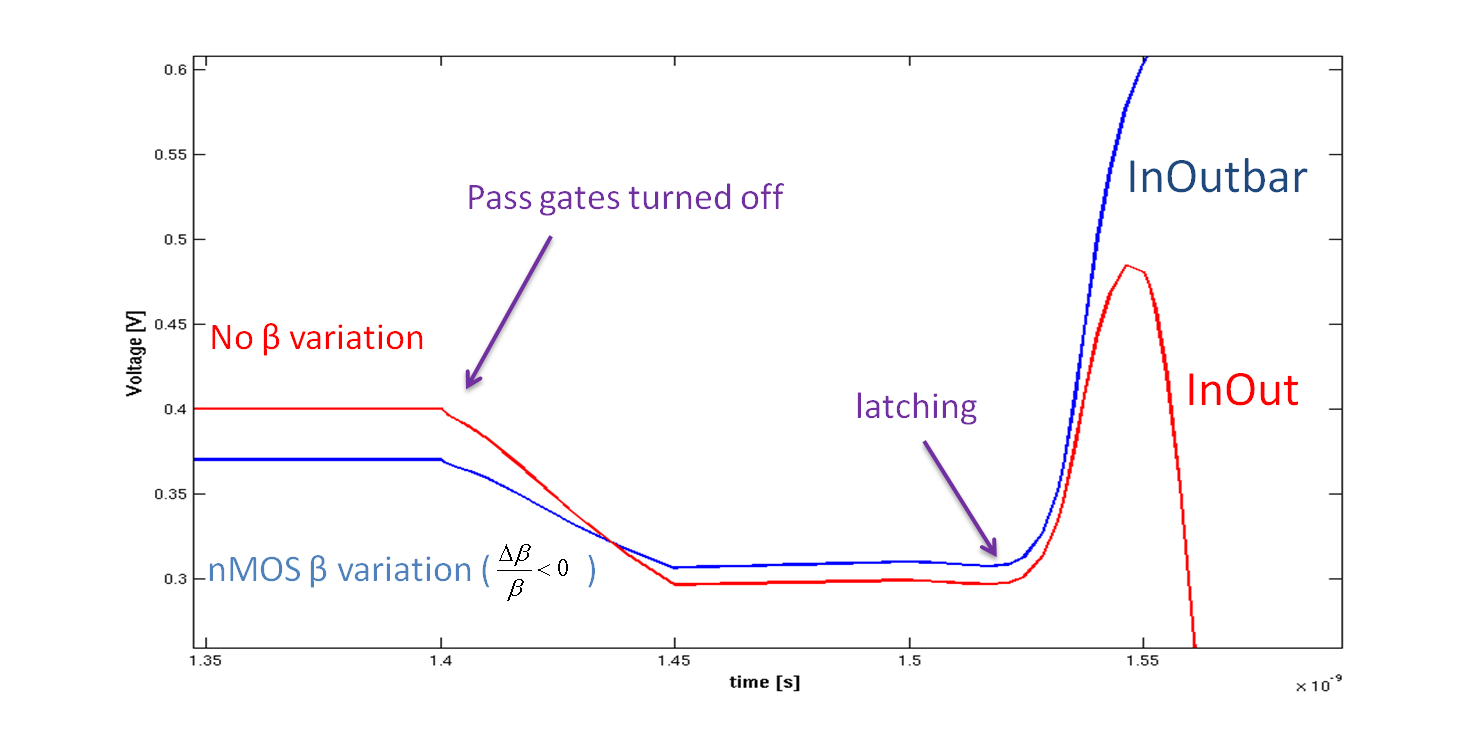
\includegraphics[scale=0.4]{../fig/hfdstk-sensamp-chargeinjectionmismatch.png}
  \caption[foutief latchen door $\beta$-mismatch]{Door $\beta$-mismatch is ladingsinjectie van de pass-gates niet meer gematched en gaat de SA foutief latchen}
  \label{fig:chargeinjectionmismatch}
\end{figure}

\subsection{RC-latch-effect}
\label{RC-latch-effect}
De situatie waarbij er volledige overlap is tussen de controle signalen kan vereenvoudigd worden opgesteld met de situatie van figuur \ref{fig:RC-latch}. De pass-gate die aanstaat wordt voorgesteld als een weerstand, de pass-gate in het local block en diens parasitaire capaciteit wordt verwaarloosd. CL bedraagt voor deze simulatie 46 fF, het equivalent voor een BL waaraan 256 cellen hangen. Cint bedraagt voor een SA met minimale transistorafmetingen 161 aF. Wanneer het dynamisch latch-gedrag bekeken wordt voor verschillende waardes van R, treedt er een merkwaardig effect op (zie figuur \ref{fig:RC-latch-sim}): voor voldoende grote waardes van R lijkt het alsof de grote capaciteit ontkoppeld is van de latch tot op een zeker tijdstip, waarna een veel tragere settling optreedt.
\begin{figure}
  \centering
  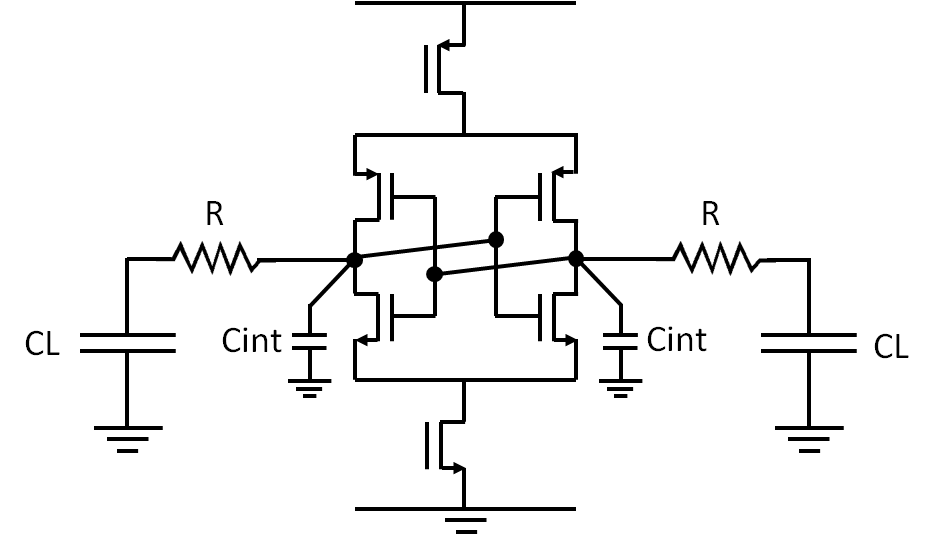
\includegraphics[scale=0.4]{../fig/hfdstk-sensamp-RC-latch.png}
  \caption[Simulatieopstelling voor het RC-latch-effect]{Simulatieopstelling voor het RC-latch-effect}
  \label{fig:RC-latch}
\end{figure}
\begin{figure}
  \centering
  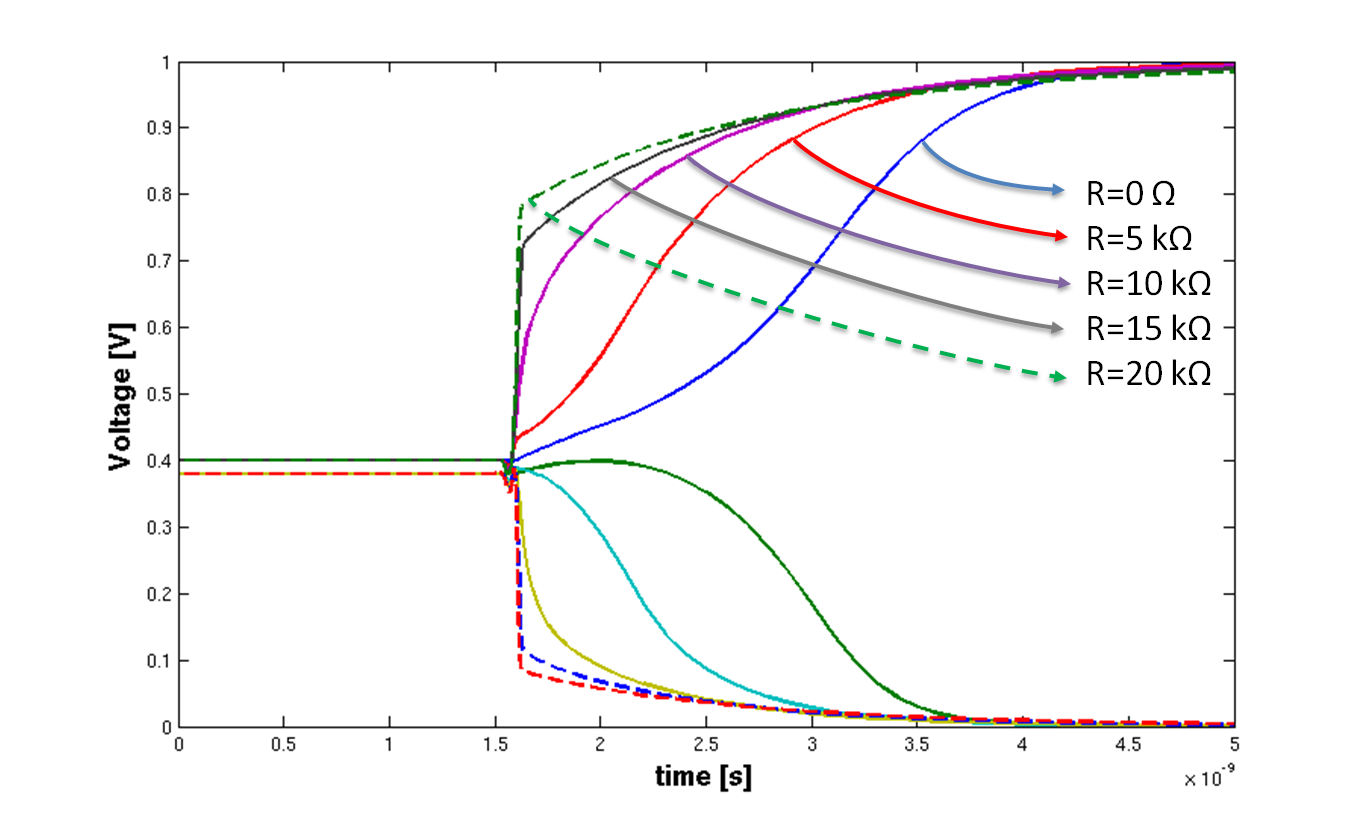
\includegraphics[scale=0.4]{../fig/hfdstk-sensamp-RC-latch-sim.png}
  \caption[Simulatieresultaten voor het RC-latch-effect]{Simulatieresultaten voor het RC-latch-effect:de 2 ingangs-uitgangsknopen zijn voorgeladen op 400mV en 380mV. Na 1,6ns wordt de SA aangezet. De SA is ideaal voor deze simulatie.}
  \label{fig:RC-latch-sim}
\end{figure}
De verklaring ligt in het feit dat CL zich voor hoge frequenties als een kortsluiting gedraagt (zie figuur \ref{fig:RC-latch-explain}), een plotse stroom vloeit door de weerstand en hierdoor onstaat er een spanningsval over de weerstand. Hierna gaat er op veel lagere frequenties een spanning beginnen op te bouwen over de capaciteit waardoor de ingangs-uitgansknopen volledig kunnen laden/ontladen tot VDD en VSS.
\begin{figure}
  \centering
  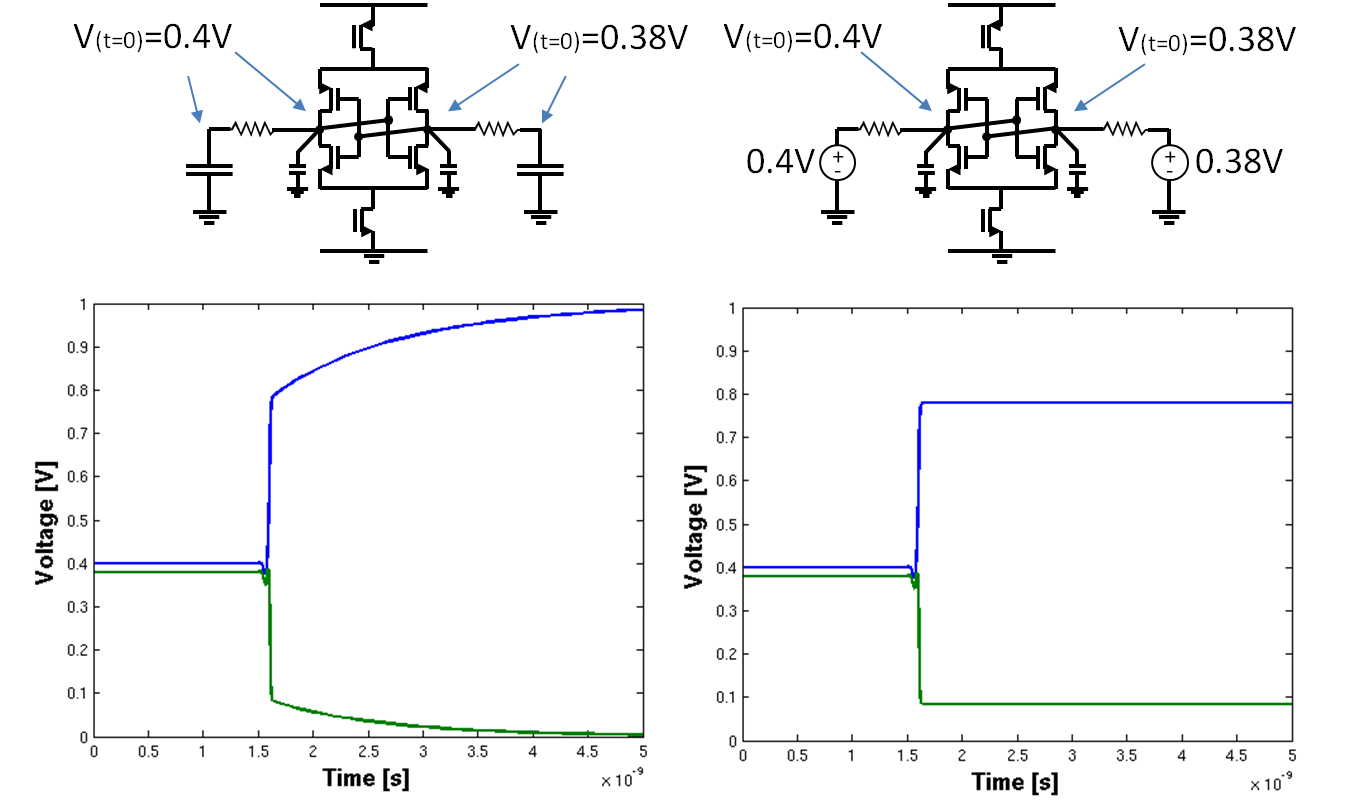
\includegraphics[width=\textwidth]{../fig/hfdstk-sensamp-RC-latch-explain.png}
  \caption[Invloed capaciteit op RC-latch effect]{Vergelijking situatie met voorgeladen (eindige) capaciteit en situatie met spanningsbron (oneindige capaciteit)}
  \label{fig:RC-latch-explain}
\end{figure}
Gevolgen van wanneer dit effect optreedt is dus dat het nuttige signaal zich snel - alsof er helemaal geen last aanhangt - en lineair opbouwt en dat er geen AC-signaal is over de condensator. Een analyse van de respons van een RC-circuit op een lineair stijgende spanningsbron geeft meer duidelijkheid voor de voorwaarden waarop het RC-latch-effect optreedt (zie figuur \ref{fig:RC-latch-maplecircuit}). De respons van de spanning over de capaciteit is $Vcap(t) =  at - aRC(1-e^{-{\frac {t}{CR}}})$. Uit deze uitdrukking blijkt dat het RC-latch-effect optreedt wanneer de latch zonder last snel is (a<<1) en/of wanneer het RC-product hoog is (RC>>1).
Wanneer het effect zich voordoet zijn latching en RC-respons onafhankelijke processen. Wanneer de voorwaarden niet meer zo uitgesproken zijn, gaan deze processen met elkaar interfereren en is het moeilijk dit gecombineerde proces wiskundig te beschrijven.
\begin{figure}
  \centering
  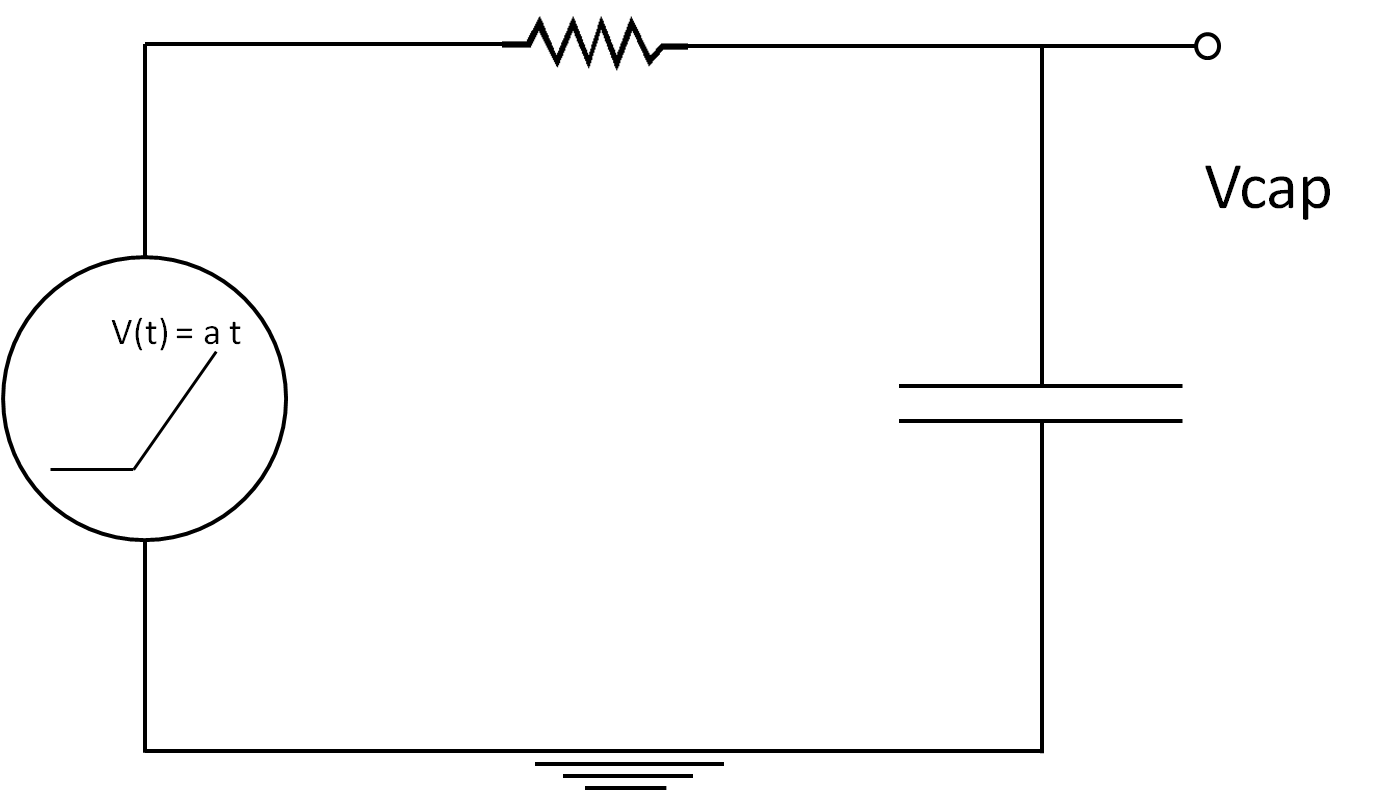
\includegraphics[scale=0.4]{../fig/hfdstk-sensamp-RC-latch-maplecircuit.png}
  \caption[Circuit voor analyse voorwaarden RC-latch-effect]{Circuit voor analyse voorwaarden RC-latch-effect}
  \label{fig:RC-latch-maplecircuit}
\end{figure}

Conclusie van het RC-latch effect is dat de timing helemaal niet zo kritisch is: in theorie hoeft de overlap slechts even lang te duren als de delay van de SA wanneer er geen last op is aangesloten, maar het is niet erg als de overlap wat langer duurt.
De pass-gates mogen ook minimaal zijn, om hun aanweerstand te vergroten zodat het effect kan optreden.
In geval verder zou gewerkt worden met een SA zonder overlap met pass-gate-enable en SA-enable, zouden de pass-gates moeten geschaald worden om de mismatch te minimaliseren. Dit zou wel betekenen dat er per schakeling van de passgates een grotere hoeveelheid lading wordt geïnjecteerd.


\subsection{Sensitiviteitsanalyse voor minimale SA - vervolg}

In tabel \ref{tab:min-sensanalysis-overlap} worden de resultaten van een nieuwe sensitiveitsanalyse getoond voor een minimale SA, ditmaal waarbij er dus overlap is tussen pass-gate-enable en SA-enable. De spreiding van de offsetspanning is wel degelijk gedaald. Toch heeft de mismatch van de passgates nog steeds een significante bijdrage, dit kan verklaard worden a.d.h. van figuur \ref{fig:RC-latch}: de 2 weerstanden zijn niet gematcht, deze mismatch treedt op door zowel $\beta$- als $V_{T}$-mismatch van de passgates. De bijdrage van de mismatch van de differentiële paren daalt echter door de interactie met de passgates.

\begin{table}
\begin{tabular}{cccccc}
\hline 
Transistor & Parameter & Richtingscoëfficiënt [$\frac{mV}{\sigma}$] & W [nm] & L [nm] & $\sigma$ \\ 
\hline 
Mupbar & Vt & 15.3 & 100 & 45 & 37.3mV \\ 
Mup & Vt & -14.9 & 100 & 45 & 37.3mV \\ 
Mdownbar & Vt & 10.3 & 100 & 45 & 42.0mV \\ 
Mdown & Vt & -9.9 & 100 & 45 & 42.0mV \\
Mpassn & $\beta$ & 8.4 & 100 & 45 & 29.8\% \\ 
Mpassbarn & Vt & 6.8 & 100 & 45 & 42.0mV \\
Mpassbarn & $\beta$ & -6.8 & 100 & 45 & 29.8\% \\
Mpassn & Vt & -6.7 & 100 & 45 & 42.0mV \\ 
Mupbar & $\beta$ & 6.4 & 100 & 45 & 17.9\% \\ 
Mup & $\beta$ & -6.1 & 100 & 45 & 17.9\% \\ 
Mdownbar & $\beta$ & -5.6 & 100 & 45 & 29.8\% \\  
Mdown & $\beta$ & 5.2 & 100 & 45 & 29.8\% \\ 
Mpassp & Vt & 0.23 & 100 & 45 & 37.3mV \\
Mpassbarp & Vt & -0.23 & 100 & 45 & 37.3mV \\
Mtop & Vt & 0.17 & 100 & 45 & 37.3mV \\  
Mpassp & $\beta$ & -0.17 & 100 & 45 & 17.9\% \\ 
Mpassbarp & $\beta$ & 0.17 & 100 & 45 & 17.9\% \\ 
Mtop & $\beta$ & 0.12 & 100 & 45 & 17.9\% \\
Mbottom & $\beta$ & 0.050 & 100 & 45 & 29.8\% \\ 
Mbottom & Vt & 0.033 & 100 & 45 & 42.0mV \\ 
\hline 
\hline & $\sigma_{Voffset}$: & 31.7mV & & & \\
\hline
\end{tabular} 
\caption[Sensitiviteitsanalyse van de minimale SA met overlap tussen passenable en latchenable]{Sensitiviteitsanalyse van de minimale SA met overlap tussen passenable en latchenable}
\label{tab:min-sensanalysis-overlap}
\end{table}

\subsection{Sensitiviteitsanalyse voor gebruikte SA}

In tabel \ref{tab:ourSA-sensanalysis-overlap} worden de resultaten van een sensitiviteitsanalyse getoond voor de SA die gebruikt wordt in het finale geheugenontwerp. Deze is gekozen aan de hand van de resultaten van de paretosimulatie in de volgende sectie.


\begin{table}
\begin{tabular}{cccccc}
\hline 
Transistor & Parameter & Richtingscoëfficiënt [$\frac{mV}{\sigma}$] & W [nm] & L [nm] & $\sigma$ \\ 
\hline 
Mup & Vt & -4.3 & 1700 & 45 & 9.0mV \\ 
Mupbar & Vt & 4.3 & 1700 & 45 & 9.0mV \\ 
Mpassn & Vt & -3.8 & 500 & 45 & 18.8mV \\
Mpassbarn & Vt & 3.7 & 500 & 45 & 18.8mV \\
Mpassbarn & $\beta$ & -3.0 & 500 & 45 & 13.3\% \\ 
Mpassn & $\beta$ & 3.0 & 500 & 45 & 13.3\% \\ 
Mup & $\beta$ & -1.8 & 1700 & 45 & 4.3\% \\ 
Mupbar & $\beta$ & 1.8 & 1700 & 45 & 4.3\% \\ 
Mdown & Vt & -1.1 & 1500 & 45 & 10.9mV \\ 
Mdownbar & Vt & 1.1 & 1500 & 45 & 10.9mV \\
Mdown & $\beta$ & 0.83 & 1500 & 45 & 7.7\% \\
Mdownbar & $\beta$ & -0.83 & 1500 & 45 & 7.7\% \\  
Mpassp & Vt & 0.17 & 500 & 45 & 16.7mV \\ 
Mpassp & $\beta$ & 0.17 & 500 & 45 & 8\% \\ 
Mpassbarp & Vt & -0.17 & 500 & 45 & 16.7mV \\
Mpassbarp & $\beta$ & -0.17 & 500 & 45 & 8\% \\ 
Mtop & $\beta$ & 0.13 & 900 & 45 & 6.0\% \\ 
Mtop & Vt & 0.10 & 900 & 45 & 12.4mV \\ 
Mbottom & $\beta$ & -0.067 & 500 & 45 & 13.3\% \\ 
Mbottom & Vt & 0.033 & 500 & 45 & 18.8mV \\ 
\hline 
\hline & $\sigma_{Voffset}$: & 9.6125mV & & & \\
\hline
\end{tabular} 
\caption[Sensitiviteitsanalyse van de SA in het finale geheugen]{Sensitiviteitsanalyse van de SA in het finale geheugen, er is overlap tussen de controlesignalen}
\label{tab:ourSA-sensanalysis-overlap}
\end{table}

\section{Paretosimulatie}
In het beginstadium van het ontwerp is nog niet duidelijk wat de impedantie aan de BL wordt. Het is deze impedantie die bepaalt wat het spanningsverschil is tussen het datasignaal en het referentiesignaal aan de sense amplifier. Bovendien kan het zijn dat er midden in het ontwerp besloten wordt om een andere impedantie te kiezen om alsnog te optimaliseren naar een andere variabele.
Natuurlijk is het mogelijk om één SA te gebruiken die voor elke impedantie een correcte en snelle werking zou garanderen. Dit zou echter een verspilling zijn van energie. In deze sectie wordt een pareto-oppervlak opgesteld waarbij er voor elk spanningsverschil de snelste en energiezuinigste SA-ontwerpen worden gekozen.

\subsection{Opstelling}
Uit een verzameling van allerhande SA [dit zijn sense amplifiers waarvan de transistoren verschillend geschaald zijn - differentiële paren hebben zelfde afmetingen] worden enkel de pareto-optimale SA uitgekozen. De pareto-criteria zijn $\Delta V$, snelheid en dynamische energie. 

Voor deze opstelling worden de pass-gates weggelaten van de SA [dit is geoorloofd zoals bleek uit de sensitiviteitsanalyse], de last aan de ingangs-uitgangsknopen is een simpele CMOS inverter. De knopen zijn voorgeladen op 2 spanningen: 0,4V en 0,4V - $\Delta V$. Na 0,5ns wordt de SA aangezet en wordt de tijd gemeten tot wanneer de ingangs-uitgangsknopen geladen of ontladen zijn tot 99,9\% van hun finale waarde (VDD of VSS). Dit is wellicht een te strenge methode om de snelheid van de SA te bepalen aangezien de inverters al eerder zullen schakelen. Indien de snelheid van de 2 knopen verschilt, zal de traagste tijd genomen worden. De dynamische energie wordt opgemeten van het moment dat de SA wordt aangeschakeld tot dit tijdstip. Ook het statisch vermogen van de SA wordt opgemeten wanneer de ingangs-uitgangsknopen VDD en VSS bereikten. Uiteraard wordt ook geverifieerd ofdat de SA wel correct heeft gelatcht.

Per sense amplifier worden er 250 Monte Carlo simulaties gedaan met deze opstelling. Indien de SA niet elke keer correct functioneerde, wordt de SA verworpen. Latchte de SA wel elke keer correct, wordt het gemiddelde van de delay, dynamische energie  en statisch vermogen opgeslagen. 

\subsection{Resultaten}
Op figuur \ref{fig:pareto} zijn de pareto-optimale resultaten getoond van de groep sense amplifiers. Het doel van deze simulatie is veeleer om de transistorafmetingen te situeren in functie van deze optimalizatievariabelen. Voor deze simulatieopstelling kan men enkel zeggen dat de kans dat de offsetspanning lager is dan $\Delta V$ minstens $1 -\frac{1}{250}$ is. Dit is een veel te kleine garantie voor een sense amplifier die misschien wel miljoenen keren zal gefabriceerd worden. Voor meer informatie over de verdeling van de offsetspanning te krijgen moet de standaardafwijking berekend worden met de sensitiviteitsanalyse.

\begin{figure}
  \centering
  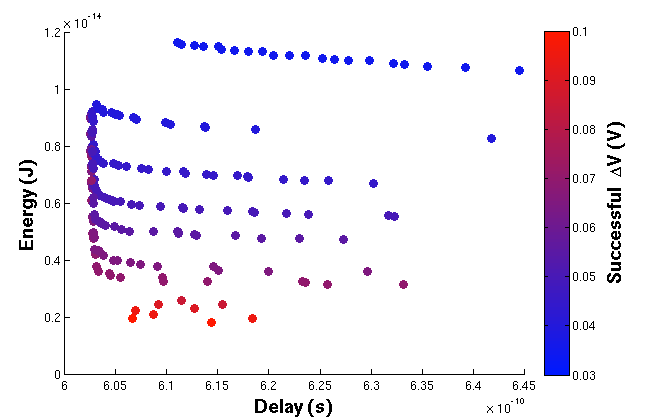
\includegraphics[width=0.8\textwidth]{../fig/hfdstk-sensamp-pareto2.png}
  \caption[De pareto-optimale sense amplifiers]{De pareto-optimale sense amplifiers}
  \label{fig:pareto}
\end{figure}

\section{Besluit}
In dit hoofdstuk werd dieper ingegaan op de sense amplifiers, die het kleine spanningsverschil tussen datasignaal en referentiesignaal correct moet versterken tot VDD en VSS. De belangrijkste eigenschap van de SA is de offsetspanning door transistorvariaties. Deze kan voldoende klein gemaakt worden door de transistoren voldoende op te schalen. De offsetspanning kan statistisch beschreven worden met behulp van een sensitiviteitsanalyse. Tenslotte worden er ook uit een grote groep SA de pareto-optimale gekozen. De resultaten geven een idee van de grootteordes van transistorafmetingen voor een bepaalde offetspanning, snelheid en dynamische energie.
